\chapter{Learning uncertainty tubes via recurrent neural networks} \label{chap:NN}
\markboth{Learning uncertainty tubes via recurrent neural networks}{}% To set left/right header
% \localtableofcontents

% Parallelization of ODE (Ordinary Differential Equations) solvers for systems like a quadrotor is indeed possible, but it comes with certain challenges due to the inherent sequential nature of ODE solvers. Each time step generally depends on the previous one, making it difficult to parallelize directly. However, various techniques and strategies can help in parallelizing ODEs, even for small time steps. Let's explore this in more detail.
% 1. Parallelization in ODE Solvers

% ODE solvers like Runge-Kutta, Euler, or Adams-Bashforth typically compute solutions in a time-stepping manner, where each step depends on the solution from the previous step. This sequential dependency makes it hard to directly parallelize time integration.

% However, some strategies can parallelize parts of the problem:
% 1.1 Parallelizing the Evaluation of Derivatives

% The right-hand side (RHS) of the ODE system (i.e., the function that describes the system's dynamics) can often be parallelized if it involves multiple independent computations. For example, in a quadrotor, if the dynamics involve complex matrix operations, vector algebra, or sensor models, these computations can be parallelized across multiple cores or even on a GPU.
% 1.2 Domain Decomposition for Parallelization

% This approach involves splitting the physical domain or the variables of the system and solving them in parallel. For a quadrotor, domain decomposition may not apply as easily as it would for a large physical domain problem (like fluid dynamics), but it could still be used if the quadrotor's dynamics are complex and involve interacting subsystems. For instance, rotor dynamics, attitude control, and position dynamics could potentially be solved in parallel if they are weakly coupled.
% 1.3 Multiple Shooting or Parareal Algorithms

% These methods introduce parallelization by splitting the time domain into multiple intervals and solving the ODE in parallel on each subinterval.

%     Parareal Algorithm: This method allows for parallel time integration by solving coarse approximations over large time intervals in parallel, followed by corrections using fine time steps. While the fine steps remain sequential, the coarse steps can be parallelized. The Parareal method is well-suited for large-scale systems but might be overkill for small systems like a quadrotor, especially with small time steps.

%     Multiple Shooting: In this technique, the time domain is divided into smaller intervals, and the ODE is solved independently in each interval. The solutions are then stitched together using boundary conditions. This method is typically used for stiff ODE problems or optimization-based control (like Model Predictive Control).

% 1.4 Parallel Integration of Different States

% In some cases, the state variables of a system might evolve independently or with weak coupling, allowing for parallel integration of different states. For a quadrotor, some aspects of the dynamics (e.g., attitude and position) could potentially be integrated separately in parallel, especially if the time scales are slightly different.
% 2. Time-Stepping Constraints and Relaxation

% You mentioned time-step constraints. In ODE solvers, especially explicit solvers like Runge-Kutta or Euler, the time step size is usually limited by stability constraints (e.g., Courant-Friedrichs-Lewy (CFL) condition for PDEs or step size for stiff ODEs).

%     Relaxing Time-Step Constraints: Parallelization techniques like Parareal introduce time-step relaxation by allowing coarse-grain parallel computations over larger time intervals, then correcting with smaller steps sequentially. This is useful for accelerating convergence in large-scale simulations with longer time horizons.

%     Using Small Time Steps in Parallelization: If your goal is to maintain small time steps (e.g., for accuracy, stability, or real-time control in a quadrotor), relaxation-based methods might not be as helpful. However, parallelization can still help in other ways:
%         Task-based Parallelism: Use parallel computing resources to speed up the evaluation of forces, torques, control inputs, sensor models, or optimization procedures (if using real-time control).
%         Predictor-Corrector Methods: These methods can use a fast, coarse-grained predictor step, followed by parallel corrections that refine the solution. The corrections can be done in parallel with small time steps, making it more suitable for small time steps.
%         Parallelization of Subsystems: Parallelizing distinct components of the quadrotor's dynamics (e.g., thrust dynamics, rotational dynamics, or environmental interactions) can improve computational efficiency while keeping the same small time steps.

% 3. Maintaining Small Time Steps in Parallelization

% To directly answer your question, you can use parallelization techniques while keeping small time steps, but the degree of parallelization might be more limited compared to approaches where time steps are relaxed. The most promising approaches in this scenario would be:

%     Parallel evaluation of the system's dynamics: Evaluating the dynamics (i.e., the forces and moments) in parallel could reduce computation time significantly, especially if your quadrotor model involves complex dynamics (e.g., aerodynamic drag, rotor dynamics, etc.).

%     Task-level parallelism: In real-time control applications, parallelizing sensor fusion, state estimation, and control computations (while maintaining small time steps) can improve performance.

%     Multiple shooting methods: Even with small time steps, the multiple shooting method can potentially parallelize certain segments of the time domain, but you'd need to stitch together the results carefully, ensuring stability.

% Conclusion

% While parallelization techniques like Parareal or Multiple Shooting often involve relaxing time-step constraints, it is still possible to parallelize certain parts of the quadrotor's ODE solver without relaxing the small time-step constraints. You can achieve this by focusing on parallelizing the evaluation of the system's dynamics, using task-level parallelism, or exploiting weakly coupled subsystems. However, the benefit of parallelization will likely be more constrained compared to systems where time-step constraints are relaxed.

% 3. Challenges of Using Parareal for Control Stability

% The Parareal method works by first running a coarse-grained simulation with larger time steps, followed by corrections using finer time steps. If the coarse solver uses large time steps, it could violate the control stability requirements during the initial stages of the Parareal iterations. This would make it unsuitable for real-time control if the initial approximation (coarse solver) is far from accurate, as the control system relies on frequent updates.



% Your GRU (Gated Recurrent Unit) neural network might be faster than other methods for solving an ODE on a CPU for several reasons related to its structure and the way neural networks handle data. The efficiency of GRU in this context largely depends on the number of operations it performs and how well it's optimized for CPU computations. Let's break it down:
% Why GRU is Faster for ODE Solving on CPU:

%     Fewer Parameters: GRUs are known for their simplicity compared to other recurrent neural networks (RNNs) like LSTMs. GRUs have fewer gates and parameters, making them computationally cheaper.
%         GRUs have only two gates (reset and update), while LSTMs have three gates (input, forget, output), which translates to fewer matrix multiplications per time step.
%         Fewer parameters also mean less memory consumption, which reduces the computational load when training or running the model.

%     Parallelism: Neural networks, including GRUs, can be structured in such a way that they process multiple data points (or time steps) in parallel, especially during training or inference. This can make GRUs more efficient than traditional methods for solving ODEs, such as Runge-Kutta, which might be more sequential in nature.

%     Reduced Complexity of Time-Stepping:
%         Numerical methods for solving ODEs, such as Runge-Kutta or implicit methods, often involve multiple function evaluations at each time step. GRUs, however, learn a representation of the system's dynamics, effectively "learning" a function approximation, which can be faster at runtime.
%         GRUs can use a single pass per time step (or batch of time steps), while traditional solvers may require many steps or iterations at each point.


% Model Type	Inference Time	Remarks
% RNN (GRU, LSTM)	Faster	Efficient for discrete, regular time steps; fixed computation per time step
% Neural ODE	Slower	Inference depends on ODE solver complexity and system dynamics

% In most practical scenarios, RNNs (GRUs, LSTMs) will offer faster inference compared to Neural ODEs due to the absence of ODE solvers and the simpler, more direct nature of their computations. Neural ODEs are more suited for scenarios where continuous dynamics are the priority, but this often comes at the cost of slower inference times.

% Time Steps vs. ODE Solver Integration:

%     In RNNs, the number of time steps is fixed, and you perform one forward pass per time step.
%     In Neural ODEs, the time steps are determined by the ODE solver, which can be adaptive. The solver may take many small steps or fewer large steps, depending on the system's complexity.

%     RNNs (GRU, LSTM, etc.):

%     RNNs are designed to handle discrete time sequences. They take input in the form of a time series with fixed time steps (e.g., t1,t2,t3,...) and learn to map these discrete states over time.
%     RNNs operate by passing hidden states from one time step to the next, effectively modeling the temporal correlations in the data.
%     LSTMs and GRUs are specific variants of RNNs that improve on the basic RNN structure by addressing the problem of vanishing/exploding gradients in long sequences. They do this using gating mechanisms that control the flow of information through time.
%     Since RNNs work with fixed time steps, they model time as discrete, and handling continuous dynamics requires fine-tuning, such as choosing a time step size.

% Neural ODEs:

%     Neural ODEs, on the other hand, model continuous-time dynamics. They replace the discrete sequence of states (as in RNNs) with a differential equation for the hidden states:
%     dh(t)dt=f(h(t),t,θ)
%     dtdh(t)=f(h(t),t,θ) where ff is a neural network and θθ are its parameters. The dynamics evolve continuously over time, and you can evaluate the state at any arbitrary time tt, not just at predefined discrete steps.
%     Neural ODEs use ODE solvers to numerically integrate the system over time, allowing for flexible handling of varying time steps and even irregular or non-uniform time intervals.


% The use of a simple GRU architecture instead of Neural ODEs or Physics-Informed Neural Networks (PINNs) to approximate ODE solutions in the context of the paper by Wasiela et al. likely stems from several practical advantages that GRUs offer, particularly in the domain of real-time robot motion planning and control. Here are the key reasons and advantages of this choice:
%     1. Efficiency and Simplicity in Real-Time Applications
    
%     GRUs are known for their computational efficiency, especially in real-time applications like robotics where fast decision-making is crucial. A GRU-based model can be trained relatively easily and deployed quickly for inference, allowing the robot to plan and adjust its motions on the fly.
    
%         Fewer Parameters: Compared to models like Neural ODEs or more complex recurrent architectures, GRUs have a simpler structure and fewer parameters, making them faster and more efficient during inference. This makes GRUs particularly well-suited for tasks where real-time performance is required, such as robot motion planning.
    
%     2. Handling Sequential Data with Temporal Dependencies
    
%     GRUs are designed to handle sequential data and are efficient at modeling temporal dependencies, which are common in dynamical systems. In the context of approximating ODEs for robot motion, where states evolve over time, GRUs can track the evolving state of the robot and make predictions about future states efficiently.
    
%         Unlike Neural ODEs, which require solving differential equations iteratively through a solver, GRUs can directly approximate the state transitions (i.e., how the system evolves in time) in a single forward pass per time step, making them faster for inference.
    
%     3. Avoiding the Complexity of ODE Solvers
    
%     Neural ODEs, while powerful, often rely on the use of ODE solvers during training and inference, which can be computationally expensive and require adaptive step sizes. These solvers often need to balance accuracy with computational speed, which can become a bottleneck in real-time applications.
    
%         GRUs, in contrast, do not require iterative solvers to propagate forward in time. Once trained, a GRU can generate the next state in the sequence in a single step, leading to much faster performance, especially in resource-constrained environments like robotics.
    
%     4. Flexibility and Generalization
    
%     GRUs are flexible in terms of what kind of sequential data they can handle. Unlike Physics-Informed Neural Networks (PINNs), which integrate physical constraints directly into the learning process (requiring knowledge of the system’s physics and explicit boundary conditions), GRUs can approximate ODEs without needing explicit knowledge of the underlying physical laws.
    
%         This makes GRUs a more flexible and practical choice when the goal is to approximate the system’s behavior based on empirical data, rather than being strictly bound to physical laws or differential equations. This is especially useful in real-world scenarios where the system dynamics may be complex or partially unknown.
    
%     5. Data-Driven Approach with Learned Dynamics
    
%     In applications where data-driven approaches are preferred (such as when the robot's environment is highly dynamic or uncertain), GRUs can learn to model the system’s dynamics based purely on input-output data without needing a detailed mathematical model.
    
%         Neural ODEs and PINNs require knowledge of the system’s governing equations (or their differential form), which may not always be available or easy to define in the context of robot motion planning with uncertainties. A GRU can capture complex non-linear dynamics without needing to explicitly model the differential equations.
    
%     6. Handling Uncertainty and Robustness
    
%     In the paper, the GRU is used to model Learned Uncertainty Tubes, which suggests that the authors are dealing with uncertain environments and need a way to account for this uncertainty in planning robust robot motions. GRUs are good at capturing uncertainty in sequential predictions because of their inherent ability to model and propagate information over time.
    
%         GRUs can be trained to model not just the system's trajectory, but also the potential deviations or uncertainties in future states. This allows the GRU-based model to handle uncertain environments more robustly and efficiently, which may be harder to achieve with Neural ODEs or PINNs due to the complexity of integrating uncertainty into those frameworks.
    
%     7. Empirical Success and Ease of Implementation
    
%     Another reason for choosing GRUs could simply be their empirical success in time-series forecasting and modeling dynamic systems. They are widely used and have proven to work well in practice. Additionally, GRUs are easier to implement and train compared to Neural ODEs or PINNs, which often require more sophisticated training setups, custom loss functions, and solvers.
%     Summary of Advantages of Using GRUs over Neural ODEs or PINNs:
    
%         Faster inference: GRUs don't need iterative ODE solvers, making them more efficient for real-time applications.
%         Simplicity: GRUs are simpler to implement and require fewer resources compared to Neural ODEs or PINNs.
%         Good at handling sequential data: GRUs excel at modeling time-series data and can approximate temporal dependencies effectively.
%         Data-driven and flexible: GRUs can approximate the dynamics of a system without needing a detailed mathematical model of the underlying physics.
%         Handling uncertainty: GRUs are well-suited for modeling uncertainty in robot motion planning, as they can track evolving dynamics and uncertainties over time.
    
%     By using GRUs, the authors likely balance between achieving real-time performance, modeling complex dynamics, and managing uncertainties—all essential for robust robot motion planning.

%     You're absolutely right. Since the authors in the mentioned paper want to bypass the ODEs and avoid calling traditional solvers (like Euler, Runge-Kutta, etc.), Neural ODEs (NODEs) are not suitable because NODEs inherently rely on ODE solvers during inference. Let's now consider whether Physics-Informed Neural Networks (PINNs) could be an alternative, given the situation.
%     Why PINNs Might Not Be the Right Fit in This Context
    
%     Even though PINNs integrate known ODEs into the learning process, there are several reasons why they might not be the best choice for this particular case where the authors want to completely bypass the ODEs:
    
%     2. PINNs May Not Be as Efficient in Real-Time
    
%         PINNs often require more computational resources and longer training times because they solve ODEs in a way that enforces the governing equations (through residuals and constraints). This can lead to slower inference times compared to using something like a GRU, which is purely data-driven and bypasses both the explicit and implicit use of ODEs.
    
%         In the context of robot motion planning—which requires fast, real-time predictions—PINNs might be overkill or too computationally demanding for the purpose, especially when the focus is on efficient approximation of motion without solving differential equations explicitly.
    
%     3. PINNs Are Better Suited When Physics Constraints Are Critical
    
%         PINNs excel when you want to incorporate physical constraints or laws explicitly during learning, particularly when data is sparse or noisy. However, in the case where the authors want to approximate the ODEs using a simple data-driven approach (like a GRU), it suggests that they are prioritizing speed and simplicity over strict adherence to the physics.
    
%         If the authors are confident that the GRU can capture the dynamics without relying on the exact physical laws during inference, then the use of PINNs—which are designed to enforce those physical laws—becomes unnecessary.

\section{Reccurent neural networks: overview}

\section{Method} \label{sec:method}

This section presents a multi-task learning neural network based on a GRU architecture, which takes as input the desired states of the dynamic system and outputs the nominal control inputs $\u_n$, as well as the uncertainty tubes around the states $\Rq$ and the control inputs $\Ru$. 

\subsection{Problem statement}

The goal is to train a neural network to approximate sensitivity-based uncertainty tubes, hence avoiding the computational cost of solving many \myglsentry{odes}. 
Moreover, the model aims at predicting the control inputs that the system will exert to successfully track a desired trajectory, in addition to the uncertainty tubes on these control inputs. 
Given a sequence of desired robot state vectors $\textbf{M} = \{\q_{d}^0, \q_{d}^1, ..., \q_{d}^n\}$ representing the desired robot's motion (i.e. a desired trajectory to follow), the task at hand is to learn a function $\boldsymbol{g}$ that estimates the radii of uncertainty tubes for each state $\q_{d}^k$ as well as the robot control inputs at this state such that:
\begin{equation}\label{eq:prob_statement}
\{\Rq^{k}, \Ru^{k},\u^{k}\} = \boldsymbol{g}(\q_{d}^0, \q_{d}^1, ... \q_{d}^{k-1})
\end{equation}
Since evaluating the function $\boldsymbol{g}$ on $\q_{d}^k$ depends on all the previous states of the robot in $\textbf{M}$, recurrent neural network architectures are a good fit given their ability to encode and accumulate temporal information while keeping inference time low.

\subsection{Neural network architecture}\label{sec:architecture}

\begin{figure} [t]
    \centering
    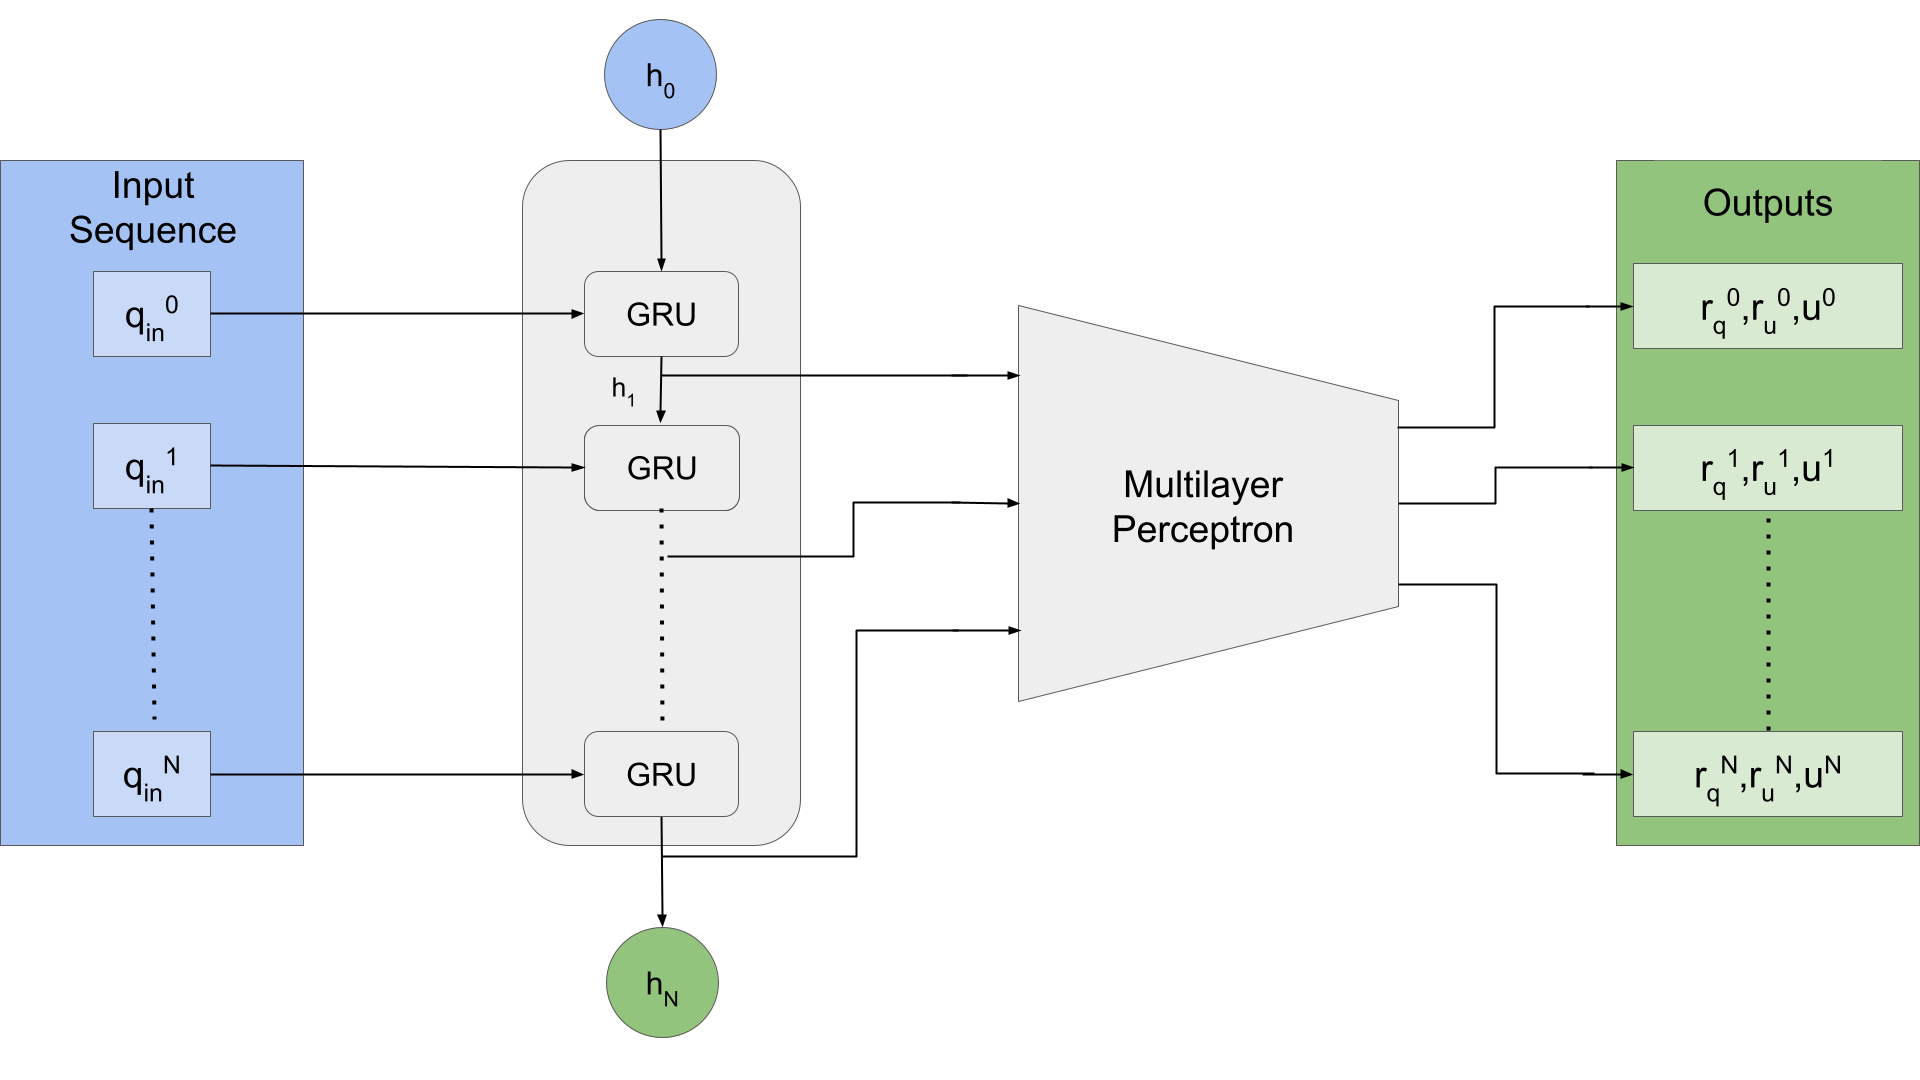
\includegraphics[width=0.8\linewidth]{figures/learning_quadrotor/SensiNN_GRU.png}%
    \caption{Representation of the proposed neural network architecture.
    }%
    \label{fig: NN}%
\end{figure}

A representation of the neural network architecture is presented in Figure~\ref{fig: NN}.
Blue blocks refer to the inputs of the model which are composed of an initial hidden state $h_{0}$ and of a sequence of desired robot states. 
For the quadrotor case, in order to make the learned model independent of workspace boundaries used during planning (i.e. robot position and orientation bounds) and initial robot orientations, only the desired linear velocities, accelerations, and yaw angular velocities ($\Dot{\Psi}_d$), are kept as the network input components.
Hence, the input to the neural network is a vector $\boldsymbol{\q_{in}^k} = [\boldsymbol{v_d} ,\, \boldsymbol{a_d} ,\, \Dot{\Psi}_d]^T$, where $k$ refers to the $k$-th state of the desired trajectory.

The outputs of the neural network correspond to the green blocks.
In the case of a quadrotor, it is composed of the predicted uncertainty tubes radii along the $\{x,y,z\}$-axis of the state $\Rq=$[$r_{x},\,r_{y},\,r_{z}]^T$, and the uncertainty tubes radii associated with the control inputs of the system $\Ru = [r_{u1},\,r_{u2},\,r_{u3},\,r_{u4}]^T$.
Moreover, the control input values $\u = [u_1 ,\, u_2 ,\, u_3 ,\, u_4]^T$ are required for the motion planning algorithm, and their computation depends on ODE forward integration (as shown in (Eq.~\ref{eq:dyna_ctrl})). Since our approach aims at eliminating the need for solving ODEs, we need to train the neural network to also predict the control inputs.
Finally, $h_{N}$ corresponds to the hidden state at the last point of our sequence (i.e., the last trajectory state).

At $k=0$, the first state in the input sequence $\boldsymbol{\q_{in}^0}$ and the initial hidden state $h_0$ are given to a single-layer GRU block with a hidden state size of 512, which outputs an updated hidden state $h_1$. 
The latter is then fed to a 3-layer multi-layer perceptron (MLP), each layer followed by a ReLU activation function except the final one, to obtain the predicted control inputs $\u^0$, the state uncertainty tubes $\Rq^0$ as well as the control uncertainty tubes $\Ru^0$. 
The updated hidden state $h_1$ is then given back to the GRU block along with the second element of the input sequence. This process is repeated for each element $\boldsymbol{\q_{in}^k}$ until all predictions are obtained.

The network is intended to be used in a sampling-based tree planner, where local trajectories are concatenated to form a global one. 
Thus, since the hidden state encodes and accumulates temporal information about the input sequence, the final hidden state $h_{N}$ of a local trajectory obtained after an iteration of a sampling-based tree planner can be saved and then given back as the initial hidden state $h_{0}$ for future local trajectories considered during the next iterations. 
Therefore, in practice, this initial hidden state is generally not null.

\subsection{Dataset}

\begin{figure} [t]
    \centering
    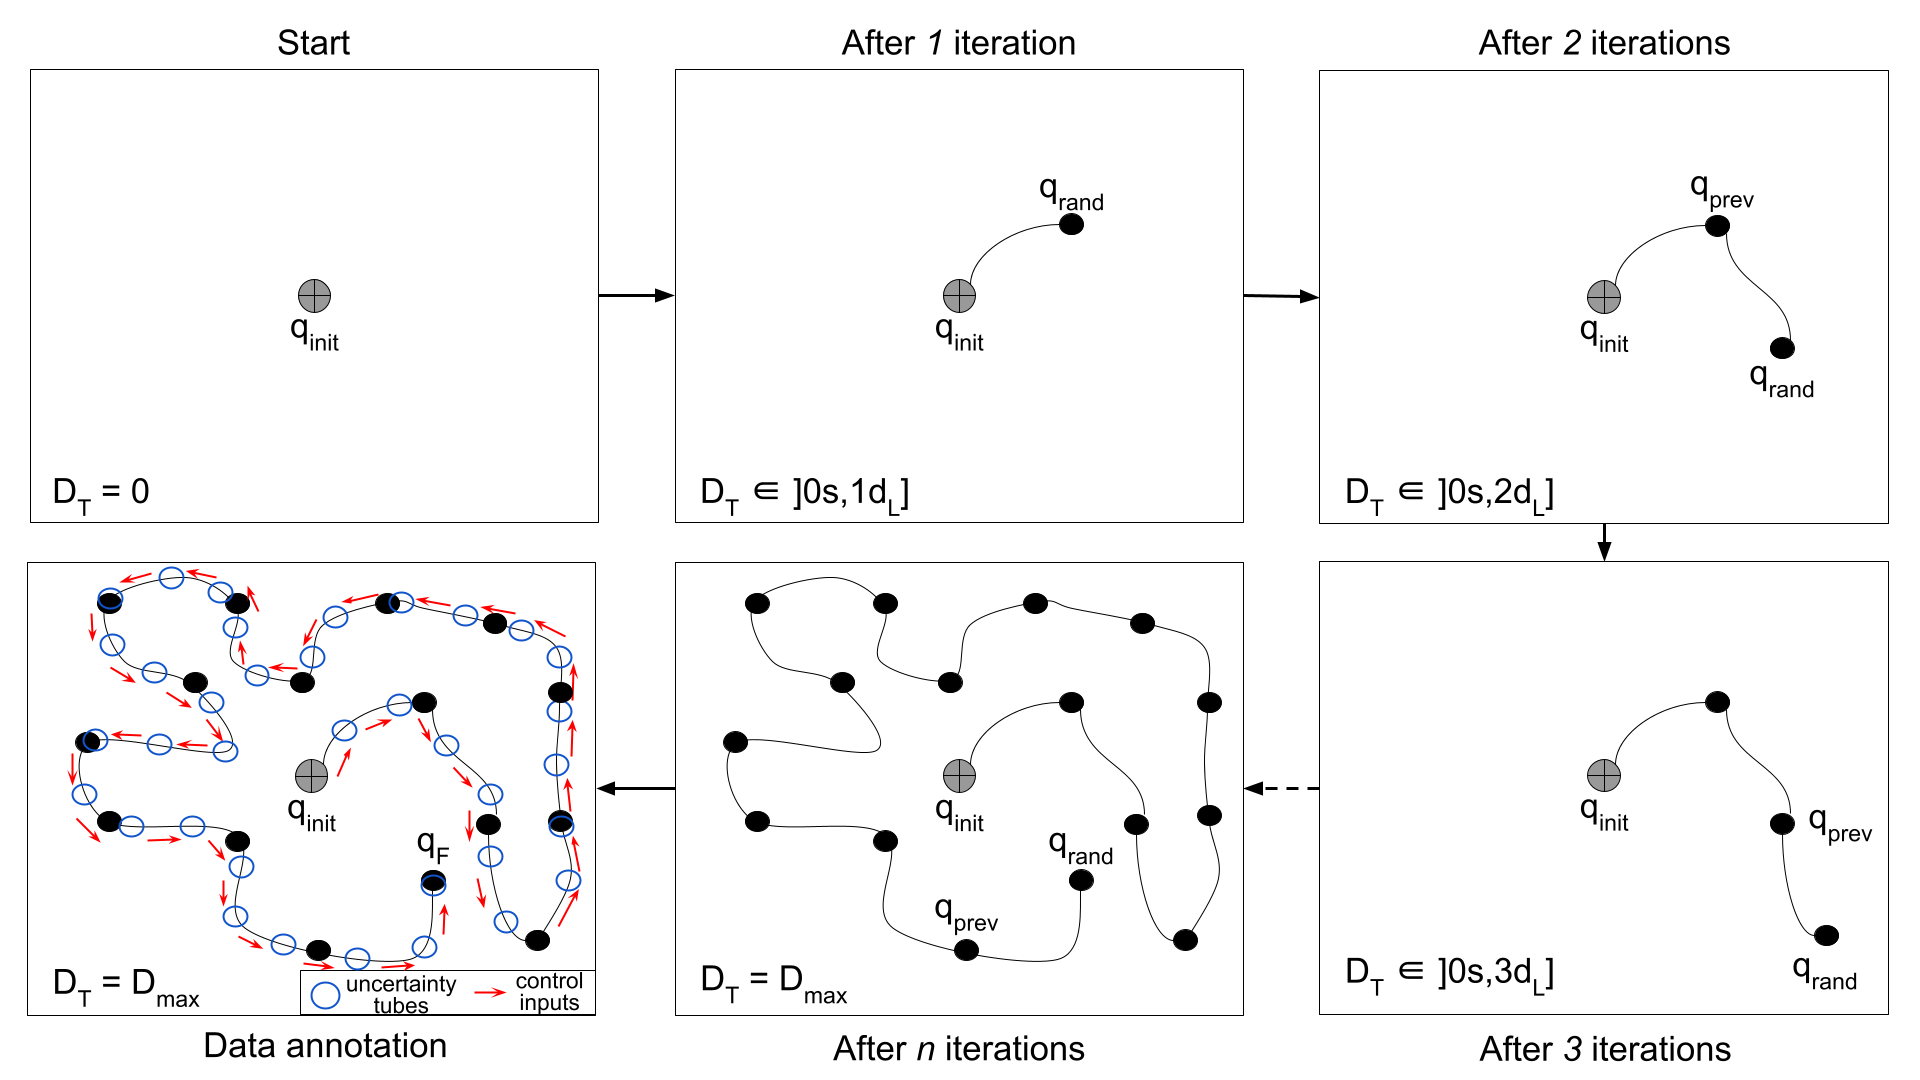
\includegraphics[width=0.9\linewidth]{figures/learning_quadrotor/dataset_generation.png}%
    \caption{Dataset generation process. 
    Starting from the hovering state $\q_{init}$, at each iteration a new state $\boldsymbol{q_{rand}}$ is randomly sampled and connected to the previous state $\boldsymbol{q_{prev}}$ until a total trajectory length ($T_F$) of 15s is reached.
    Data annotation is performed by simulating the tracking of the generated trajectory under nominal parameters.
    }%
    \label{fig: data_generation}%
\end{figure}

In order to train the proposed neural network, we generated a dataset of trajectories computed in an obstacle-free environment 
as depicted in Figure.\ref{fig: data_generation}.
This ensures that the resulting learned model is totally independent of the environment and only depends on the system.
Each global trajectory starts from the same initial hovering state ($\q_{init}$) initialized at zero velocities and accelerations\footnote{Note that this initialization does not hurt the generalizability of the model to different initial conditions and environments with obstacles (cf. Section~\ref{sec:qualitative results}).}.
Based on the same principle as a sampling-based planner, the global trajectory is made up of local sub-trajectories until a total execution time length ($T_F$) of 15s is reached.
Each local sub-trajectory is generated by uniformly sampling an arrival state ($\q_{rand}$) and connecting it to the previous sampled state ($\q_{prev}$) using a \emph{Kinosplines} steering method \cite{cKino}.
These kinosplines have the advantage of enforcing the following kinodynamic constraints on the generated splines $[v_{max}, a_{max}, j_{max}, s_{max}]$, where $v_{max},a_{max},j_{max}$ and $s_{max}$ represent the maximum allowed velocity, acceleration, jerk and snap respectively.
If the local trajectory (between $\boldsymbol{q_{rand}}$ and $\boldsymbol{q_{prev}}$) expected execution time is greater than a maximum local duration $T_l$, it is truncated to $T_l$. Similarly, when the total trajectory duration $T_F$ exceeds 15s after adding a new state, it is truncate at 15s.

To generate the outputs, i.e. to annotate the data with uncertainty tubes and control inputs, the closed-loop dynamic and the sensitivity matrices are computed by simulating the tracking of the global trajectories using an integration time step $\Delta T$ which corresponds to the same time step used for collision checking in a sampling-based motion planner.

\begin{figure} [t]
    \centering
    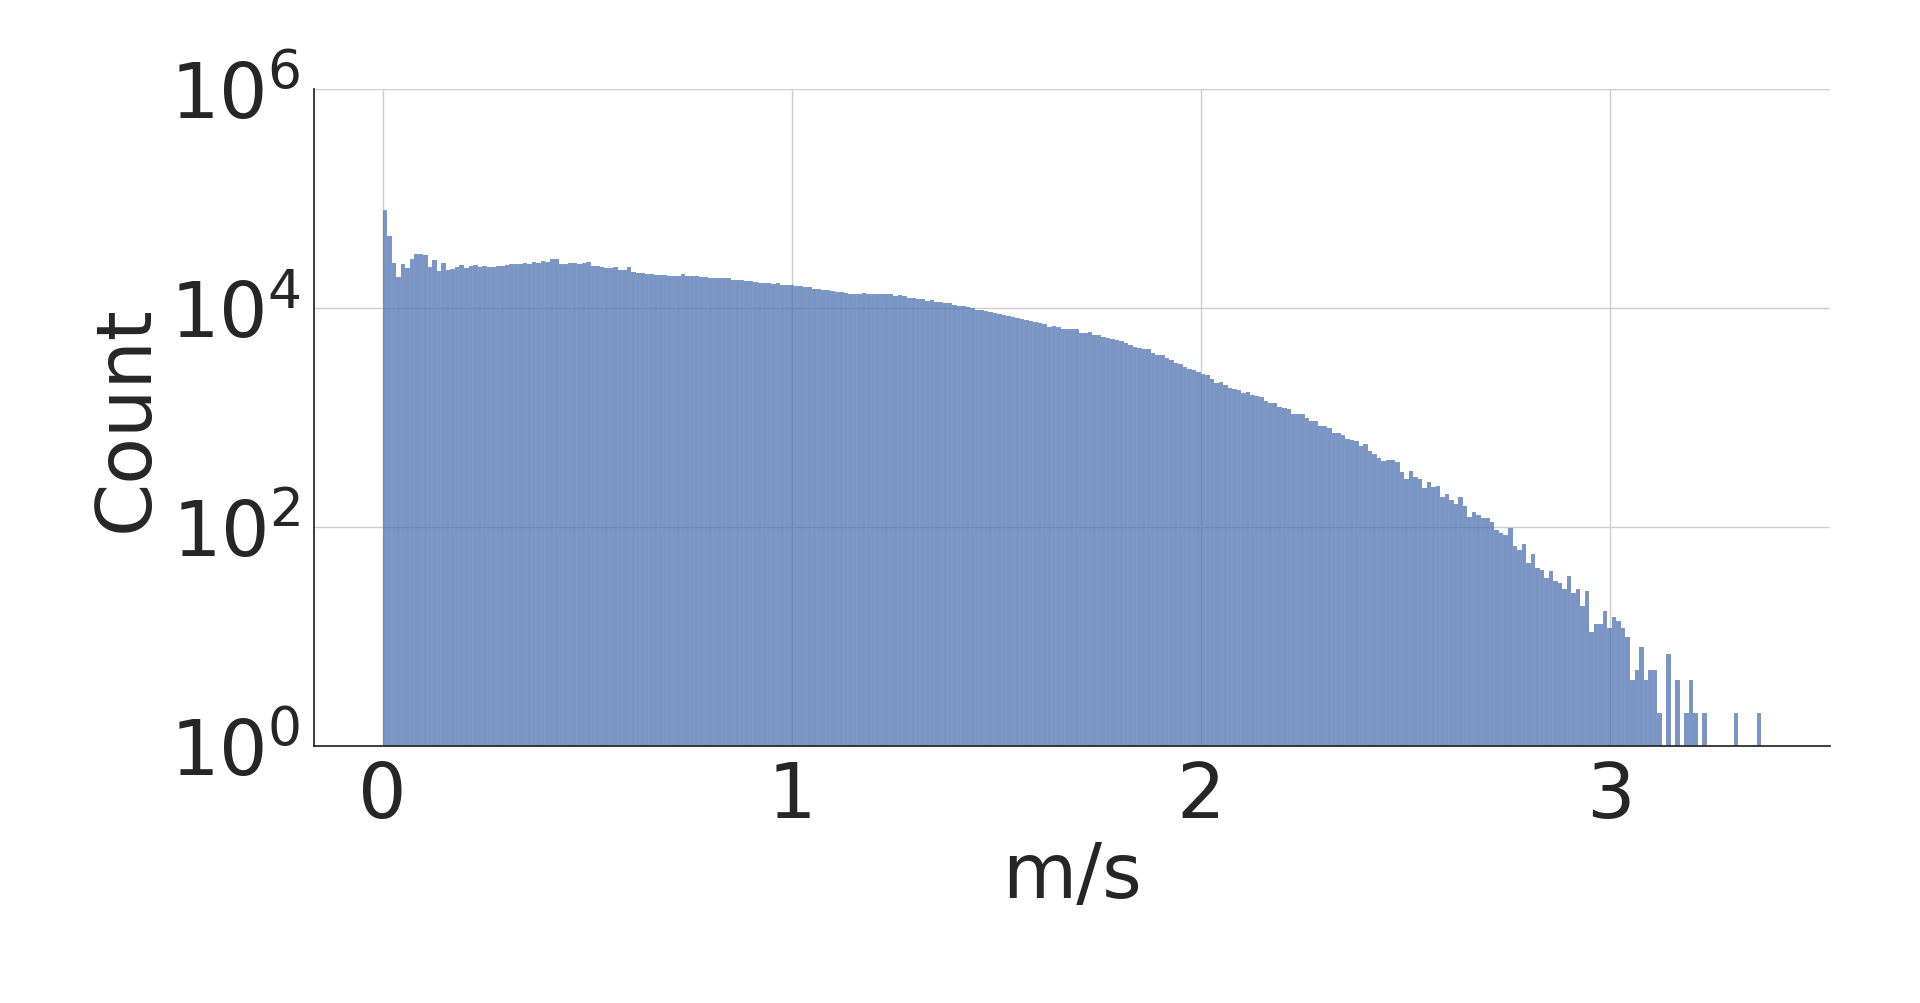
\includegraphics[width=0.49\linewidth]{figures/learning_quadrotor/vnorm_val2.png}
    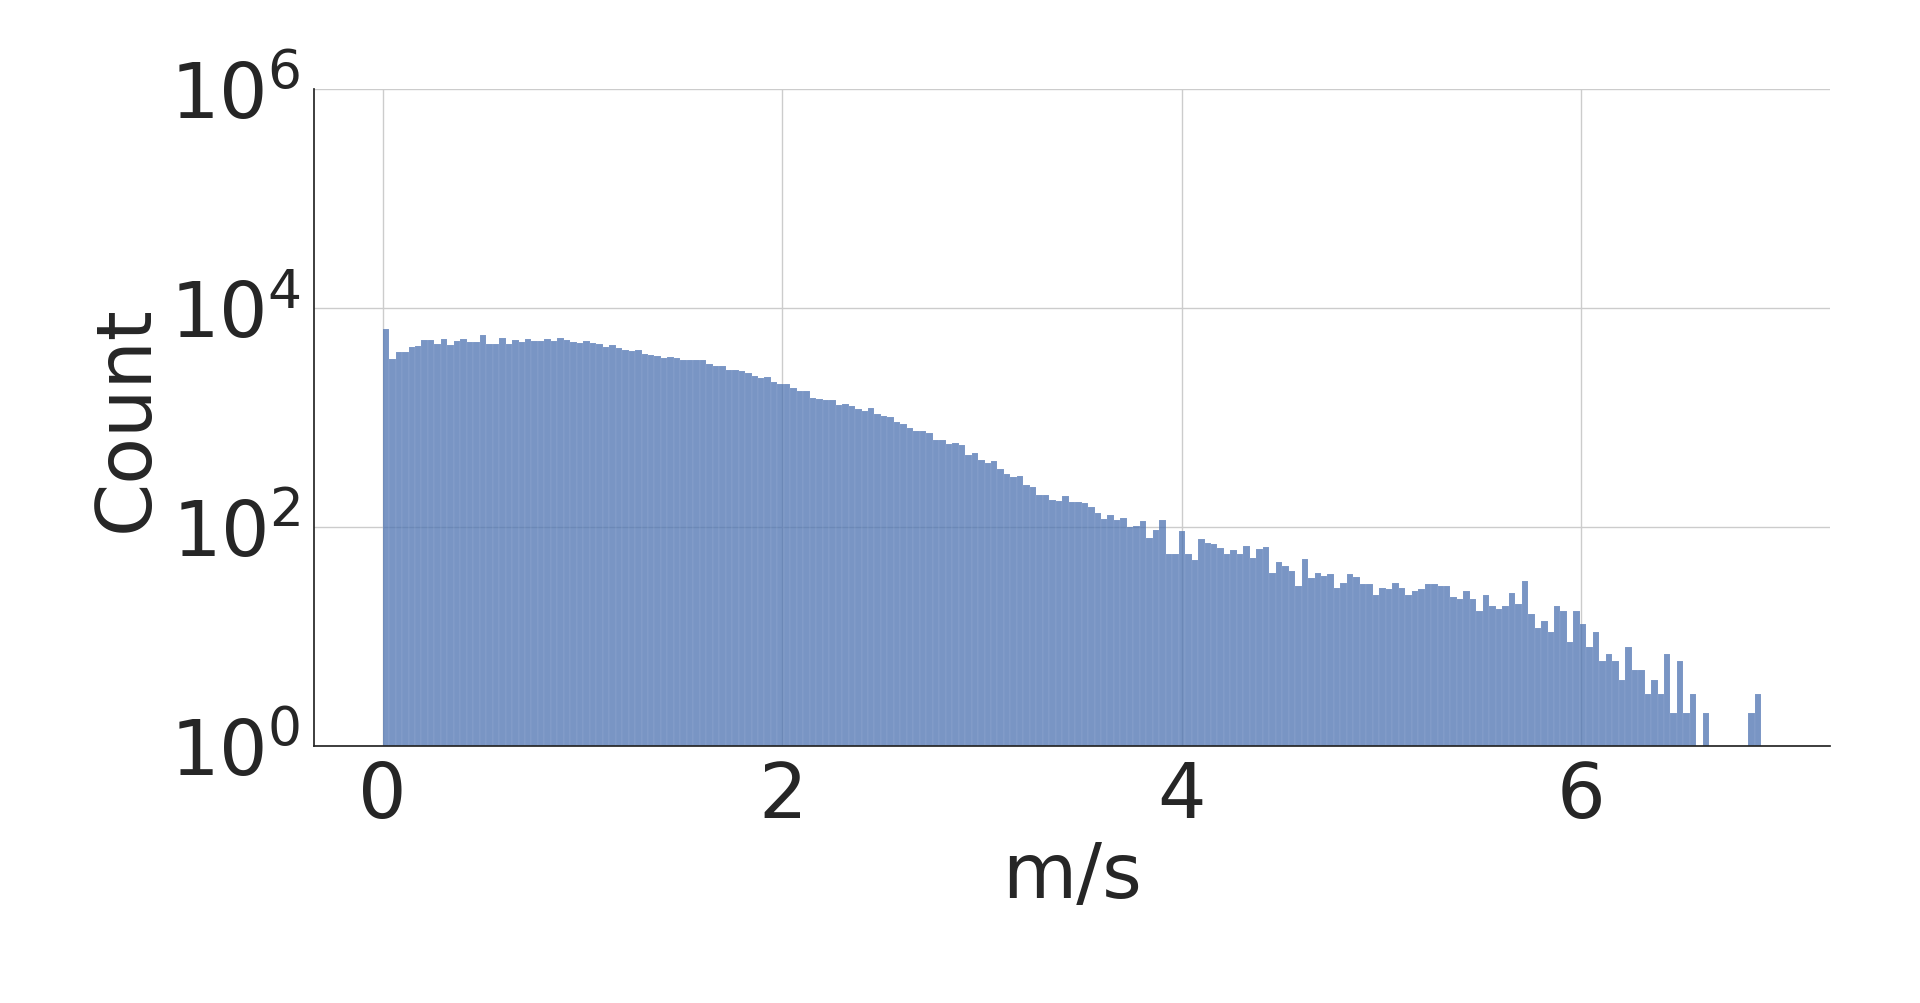
\includegraphics[width=0.49\linewidth]{figures/learning_quadrotor/vnorm_test.png}
    \caption{Velocity norm distribution in the training (left) and test sets (right).}%
    \label{fig: valvstest}%
\end{figure}
Using this mechanism, a training set composed of 8.000 trajectories and a validation set composed of 2.000 trajectories were generated, making sure that every trajectory in the dataset is different.
These trajectories were generated considering a maximum local duration of $T_l = 1s$ and an integration time step $\Delta T = 0.05s$.

The kinodynamic constraints enforced on the generated splines are $[v_{max}, a_{max}, j_{max}, s_{max}] = [5.0 \, m.s^{-1}, \allowbreak 1.5 \, m.s^{-2}, \allowbreak 15.0 \, m.s^{-3}, \allowbreak 30.0 \, m.s^{-4}]$. 
The nominal values of the uncertain parameters presented in Sect.~\ref{sec: sensi} are $\p_{c}$ = $[1.113, \allowbreak0.0, \allowbreak0.0, \allowbreak0.015, \allowbreak0.015, \allowbreak0.007]^T$ and their associated uncertainty range used for the tubes computation are $\delta\p = [7\%, \allowbreak3cm, \allowbreak3cm, \allowbreak10\%, \allowbreak10\%, \allowbreak10\%]^T$, which represents the variation of the parameters w.r.t. their associated nominal value.
The controller gains used are $\boldsymbol{k_x}=[20.0 \,, \allowbreak 20.0 \,, \allowbreak 25.0]$, $\boldsymbol{k_v}=[9.0 \,, \allowbreak 9.0 \,, \allowbreak 12.0]$, $\boldsymbol{k}_{R}=[4.6 \,, 4.6 \,, 0.8]$, $\boldsymbol{k_{\omega}}=[0.5 \,, \allowbreak 0.5 \,, \allowbreak 0.08]$.

In order to show the reliability and generalizability of the learned model, a test set composed of 1.000 trajectories was generated in the same way, but considering a maximum local duration $T_l = 2s$.
As a result, trajectories with higher velocities are encountered in the test set compared to the validation set, as depicted in Figure~\ref{fig: valvstest} where velocity norms can reach up to 7 m.s$^{-1}$ in the test set, compared with only 3 m.s$^{-1}$ in the validation set\footnote{Note that the velocity norms exceed the velocity limit $v_{max}$, this is expected since this limit applies to the components of the velocity vector rather than the norm.}.

The data annotation was performed by computing and integrating (Equation~\ref{eq:dyna_ctrl}) and (Equation~\ref{eq:dyna_sensi}) by mean of the dopri5~\cite{cdopri5} \myglsentry{odes} solver along a desired trajectory. 
Once $\bPi$ and $\bTheta$ had been computed, a simple projection was performed to recover the tubes thanks to (Eq.~\ref{eq:projection}).
Note that the control inputs $\u$ are computed during the \myglsentry{odes} resolution.
The mean and standard deviation values of the various components of the output vector for the validation and test sets generated by this setup are provided in Table~\ref{tab:datas_stats}.

\begin{table}[h]
\centering
\begin{tabular}{ | c | c || c |}
\hline
  \textbf{Output}  & \textbf{Validation set}  & \textbf{Test set} \\ \hline
$\Rq$ & $1.0e^{-1} \pm 2.0e^{-2}$ & $1.1e^{-2} \pm 2.1e^{-2}$ \\ \hline
$\u$ & $12469.3 \pm 861.6$ & $12476.8 \pm 1016.5$ \\ \hline
$\Ru$ & $7782.6 \pm 3172.3$ & $7828.6 \pm 2845.7$ \\ \hline
    
\end{tabular}
\caption{
Mean and standard deviation of the output vector components norm after data annotation for the validation and test sets.
$\Rq$ is expressed in \emph{m}, and $(\u, \Ru)$, are squared propeller angular velocities [(rad/s)²].}
 \label{tab:datas_stats}
\end{table}

\section{Evaluation}
\subsection{Metrics}

The performance of the model is evaluated using the Mean Absolute Error (MAE) over the different outputs. Rather than comparing the results on each sub-component of the input (e.g $\{x, y, z\}$ for $r_q$), we combine them into a single metric in order to obtain simpler and more general comparisons, as follows:
\begin{itemize}
    \item $\mathbf{MAE_{\Rq}}$ : represents the mean absolute error on the norm of $\Rq$. 
    For a given datapoint, given the ground truth and predicted state uncertainty tubes $\Rq$ and $\mathbf{\hat{r}_q}$, their respective norms $\|\Rq\|$ and $\|\mathbf{\hat{r}_q}\|$, are computed. 
    The mean absolute error, $\mathbf{MAE_{\Rq}}$, is then defined as:
    \begin{equation}\label{eq:MAE rq}
        \mathbf{MAE_{\Rq}} = MAE(\|\Rq\|, \|\mathbf{\hat{r}_q}\|)
    \end{equation}
    This metric is expressed in meters (m).
    \item $\mathbf{MAE_{u}}$ : represents the mean absolute error on the norm of $\u$. 
    The norms of the ground truth and predicted control inputs, $|\u|$ and $|\hat{\u}|$, are computed. 
    The mean absolute error, $\mathbf{MAE_{u}}$, is then calculated as the mean absolute error between these two norms. It is expressed in [(rad/s)²].
    \item $\mathbf{MAE_{\Ru}}$ : represents the mean absolute error on the norm of $\Ru$. As for the two previous metrics, $\mathbf{MAE_{\Ru}}$ is defined as the mean absolute error between the norms $\|\Ru\|$ and $\|\mathbf{\hat{r}_u}\|$. This metric is expressed in [(rad/s)²].
\end{itemize}

These metrics are averaged over all elements of a sequence, then averaged over all sequences in the validation and test sets. In addition, we use inference time as metric in order to evaluate the computational cost of our method compared to the defined baselines, as well as traditional uncertainty tubes computation methods involving an ODE solver. Time is denoted $T_{solver/NN}$ according to the model or solver used.

\subsection{Implementation details}

\section{Simulation results}
\subsection{Training}
\subsection{Model comparison}
\subsection{Ablation study}
\subsection{Qualitative results}

\section{Conclusion} \label{sec:NN_concl}

\todomarker{}